\documentclass[]{article}
\usepackage {amsmath}
\usepackage[a4paper, total={7.3in, 10.3in}]{geometry}
\usepackage{cleveref}

\usepackage[titletoc]{appendix}
\usepackage{lmodern}

\makeatletter
\ifcase \@ptsize \relax% 10pt
  \newcommand{\miniscule}{\@setfontsize\miniscule{4}{5}}% \tiny: 5/6
\or% 11pt
  \newcommand{\miniscule}{\@setfontsize\miniscule{5}{6}}% \tiny: 6/7
\or% 12pt
  \newcommand{\miniscule}{\@setfontsize\miniscule{5}{6}}% \tiny: 6/7
\fi
\makeatother

\usepackage{lipsum}
\usepackage{amssymb}
%\usepackage{xcolor}
\usepackage[x11names, rgb]{xcolor}
\usepackage[utf8]{inputenc}
\usepackage{mathtools}
\usepackage{xcolor}
\usepackage{braket}
\usepackage{ulem}
\usepackage{cancel}
\usepackage{graphicx}
\usepackage{mathtools}
\usepackage{amsmath}  
\usepackage{amsfonts} 
\usepackage{graphicx}
\usepackage{amssymb} 
\usepackage{amsmath}
\usepackage{mathrsfs}
\usepackage{empheq}
\usepackage{amsthm}
 \usepackage{braket}
 \usepackage{amsmath}
\DeclareMathOperator\arctanh{arctanh}
\usepackage[utf8]{inputenc}
\usepackage[english]{babel}
\usepackage{graphicx}
\newtheorem{theorem}{Theorem}[section]
\newtheorem{corollary}{Corollary}[theorem]
\newtheorem{lemma}[theorem]{Lemma}
\numberwithin{equation}{section}
\newcommand{\pd}[2]{\frac{\partial{#1}}{\partial{#2}}}
\newcommand{\Cc}{\mathbb{C}}
\newcommand{\Ss}{\mathbb{S}}
% \newcommand{\Qq}{\mathrm{q}}
\newcommand{\pT}{\hat{+}}
\newcommand{\mT}{\hat{-}}
\newcommand{\muT}{\hat{\mu}}
\newcommand{\nuT}{\hat{\nu}}
\newcommand{\alphaT}{\hat{\alpha}}
\newcommand{\betaT}{\hat{\beta}}
\newcommand{\sigmaT}{\hat{\sigma}}
\newcommand{\rhoT}{\hat{\rho}}
\newcommand{\muL}{\tilde{\mu}}
\newcommand{\nuL}{\tilde{\nu}}
\newcommand{\uniT}[1]{\mathring{#1}}
\newcommand{\itP}[1]{\hat{#1}}
\newcommand{\lF}[1]{\tilde{#1}}
\newcommand{\Pp}{\mathbb{P}}
\newcommand{\Qq}{\mathbb{Q}}
\def\epp{\epsilon^{\prime}}
\def\ep{\epsilon}
\def\vep{\varepsilon}
\def\la{\langle}
\def\ra{\rangle}
\def\ppg{\pi^+\pi^-\gamma}
\def\vp{{\bf p}}
\def\ko{K^0}
\def\kb{\bar{K^0}}
\def\ka{\kappa}
\def\al{\alpha}
\def\ab{\bar{\alpha}}
\def\be{\begin{equation}}
\def\ee{\end{equation}}
\def\bea{\begin{eqnarray}}
\def\eea{\end{eqnarray}}
\def\wh{\widehat}


\title{2D $\mathbb{Z}_2$ lattice gauge theory - Analytical solution}
\author{\textbf{Hariprashad Ravikumar}} 

\date{(For Dr. Engelhardt's meeting on Jan 12, 2023)}
\begin{document}
	\maketitle



\section{Expectation value of Wilson loop (Analytical solution)} \footnote{An introduction to lattice gauge theory and spin systems, John B. Kogut, Rev. Mod. Phys. 51, 659 – Published 1 October 1979} \footnote{ Gauge Theories of the Strong and Electroweak Interaction by Manfred Böhm , Ansgar Denner , Hans Joos, https://doi.org/10.1007/978-3-322-80160-9}\footnote{Lecture notes, A. Muramatsu- Lattice gauge theory- Summer 2009}
The expectation value of the Wilson loop $\prod_{l\in C} \sigma(l)$ is given by
\begin{align}
    \braket{\prod_{l\in C} \sigma(l)}&=\frac{\int D[\sigma]\prod_{l\in C}\sigma(l)e^{-S}}{\int D[\sigma]e^{-S}}
\end{align}
where, $S=\beta\sum_{P}(1-\sigma(\partial P))$\\
First, the Boltzmann factor for an individual plaquette is calculated, 
\begin{align}
    e^{-\beta(1-\sigma(\partial P))}=e^{-\beta}\cosh{\beta}[1+\sigma(\partial P)\tanh{\beta}]
\end{align}
The expansion of the Boltzmann factor reads 
\begin{align}
    e^{-\beta\sum_{P}(1-\sigma(\partial P))}&=\prod_{P}e^{-\beta}\cosh{\beta}[1+\sigma(\partial P)\tanh{\beta}]\\
    &=(e^{-\beta}\cosh{\beta})^{N^2}\prod_{P}[1+\sigma(\partial P)\tanh{\beta}]\\
    &=(e^{-\beta}\cosh{\beta})^{N^2}\Bigg[[1+\sigma(\partial P_1)\tanh{\beta}][1+\sigma(\partial P_2)\tanh{\beta}]\dots\dots[1+\sigma(\partial P_{N^2})\tanh{\beta}]\Bigg]\\
    &=(e^{-\beta}\cosh{\beta})^{N^2}\Bigg[[1+\tanh{\beta}\left(\sum_{G^{(1)}}\prod_{P\in G^{(1)}}\sigma(\partial P)\right)+\dots+(\tanh{\beta})^{N^2}\left(\sum_{G^{(N^2)}}\prod_{P\in G^{(n^2)}}\sigma(\partial P)\right)]\Bigg]\nonumber\\
    e^{-\beta\sum_{P}(1-\sigma(\partial P))}&=(e^{-\beta}\cosh{\beta})^{N^2}\sum_{n=0}^{N^2}(\tanh{\beta})^{n}\Bigg[\sum_{G^{(n)}}\prod_{P\in G^{(n)}}\sigma(\partial P)\Bigg]
\end{align}
then the Boltzmann
factor (partition function) is
\begin{align}
    Z &=  \int D[\sigma]e^{-\beta\sum_{P}(1-\sigma(\partial P))}\\
    &=(e^{-\beta}\cosh{\beta})^{N^2}\sum_{n=0}^{N^2}(\tanh{\beta})^{n}\Bigg[\sum_{G^{(n)}}\int D[\sigma]\prod_{P\in G^{(n)}}\sigma(\partial P)\Bigg]
\end{align}
the only non zero term in this sum is when $n=0$, i.e. $G^{(0)}$ empty lattice graph, because,
\begin{align}
    \int D[\sigma]\prod_{P\in G^{(n)}}\sigma(\partial P) = \sum_{\{\sigma \in C\}}\prod_{l\in C}\sigma(l)\sum_{\{\sigma\notin C\}}1 = 0
\end{align}
So,
\begin{align}
Z&=(e^{-\beta}\cosh{\beta})^{N^2}
\end{align}
\\
\\

Now, the numerator,
\begin{align}
    \int D[\sigma]\prod_{l\in C}\sigma(l)e^{-S}&=(e^{-\beta}\cosh{\beta})^{N^2}\sum_{n=0}^{N^2}(\tanh{\beta})^{n}\Bigg[\sum_{G^{(n)}}\int D[\sigma]\prod_{l\in C}\sigma(l)\prod_{P\in G^{(n)}}\sigma(\partial P)\Bigg]
\end{align}
here, only those $G^{(n)}$ that contribute is the one in which $\partial G^{(n)} = C$, this
is a single graph consisting of $Ar[C]$ plaquettes, where $Ar[C]$ is the number
of plaquettes which are enclosed by $C$, i.e. the area enclosed by $C$.
applies. 
\begin{figure}
    \centering
    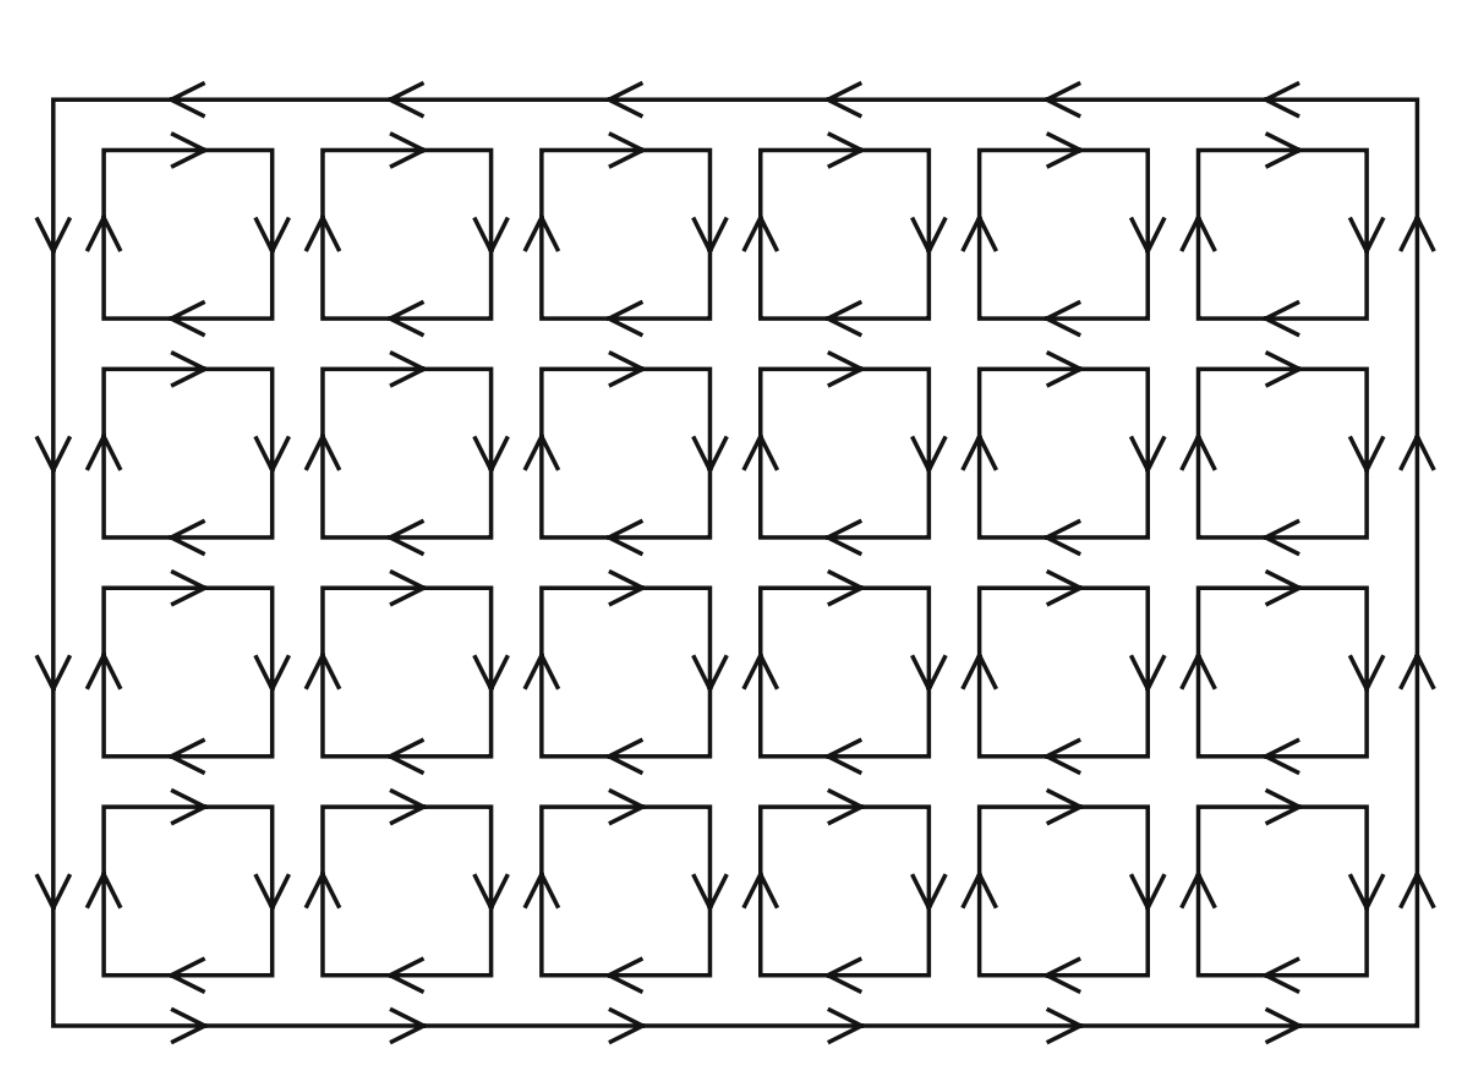
\includegraphics[scale=0.15]{IMG_DA3FC766B162-1.jpeg}
\end{figure}

Then,
\begin{align}
    \int D[\sigma]\prod_{l\in C}\sigma(l)e^{-S}&=(e^{-\beta}\cosh{\beta})^{N^2}(\tanh{\beta})^{Ar[C]}
\end{align}
Therefore,
\begin{align}
    \braket{\prod_{l\in C} \sigma(l)}&=\frac{(e^{-\beta}\cosh{\beta})^{N^2}(\tanh{\beta})^{Ar[C]}}{(e^{-\beta}\cosh{\beta})^{N^2}}\\
    &=(\tanh{\beta})^{Ar[C]}\\
    &=e^{Ar[C]\ln{\tanh{\beta}}}\\
    \Aboxed{\braket{\prod_{l\in C} \sigma(l)}&=e^{-f(\beta)Ar[C]}}
\end{align}
where
\begin{align}
    f(\beta)=-\ln{\tanh{\beta}}.
\end{align}


In our numerical calculation, the beta, $\beta=0.3$, so
\begin{align}
    f(\beta)=-\ln{\tanh{0.3}}=1.23335831883
\end{align}
\end{document}